% Copyright (C) 2014-2016 by Thomas Auzinger <thomas@auzinger.name>

\documentclass[draft,final]{vutinfth} % Remove option 'final' to obtain debug information.

% Load packages to allow in- and output of non-ASCII characters.
\usepackage{lmodern}        % Use an extension of the original Computer Modern font to minimize the use of bitmapped letters.
\usepackage[T1]{fontenc}    % Determines font encoding of the output. Font packages have to be included before this line.
\usepackage[utf8]{inputenc} % Determines encoding of the input. All input files have to use UTF8 encoding.

% Extended LaTeX functionality is enables by including packages with \usepackage{...}.
\usepackage{fixltx2e}   % Provides fixes for several errors in LaTeX2e.
\usepackage{amsmath}    % Extended typesetting of mathematical expression.
\usepackage{amssymb}    % Provides a multitude of mathematical symbols.
\usepackage{mathtools}  % Further extensions of mathematical typesetting.
\usepackage{microtype}  % Small-scale typographic enhancements.
\usepackage{enumitem}   % User control over the layout of lists (itemize, enumerate, description).
\usepackage{multirow}   % Allows table elements to span several rows.
\usepackage{booktabs}   % Improves the typesettings of tables.
\usepackage{subcaption} % Allows the use of subfigures and enables their referencing.
\usepackage[ruled,linesnumbered,algochapter]{algorithm2e} % Enables the writing of pseudo code.
\usepackage[usenames,dvipsnames,table]{xcolor} % Allows the definition and use of colors. This package has to be included before tikz.
\usepackage{nag}       % Issues warnings when best practices in writing LaTeX documents are violated.
\usepackage{hyperref}  % Enables cross linking in the electronic document version. This package has to be included second to last.
\usepackage[acronym,toc]{glossaries} % Enables the generation of glossaries and lists fo acronyms. This package has to be included last.
\usepackage{listings}

% Define convenience functions to use the author name and the thesis title in the PDF document properties.
\newcommand{\authorname}{Martin Gebhard Jenny} % The author name without titles.
\newcommand{\thesistitle}{Cloud Based Distributed Data Acquisition} % The title of the thesis. The English version should be used, if it exists.

%defines for lstlisting
\usepackage{color}
\definecolor{gray}{rgb}{0.4,0.4,0.4}
\definecolor{darkblue}{rgb}{0.0,0.0,0.6}
\definecolor{cyan}{rgb}{0.0,0.6,0.6}
\definecolor{maroon}{rgb}{0.5,0,0}
\definecolor{darkgreen}{rgb}{0,0.5,0}

\lstset{
  basicstyle=\ttfamily,
  columns=fullflexible,
  showstringspaces=false,
  commentstyle=\color{darkgreen}\upshape
}

\lstdefinelanguage{XML}
{
  basicstyle=\ttfamily,
  morestring=[s]{"}{"},
  morecomment=[s]{?}{?},
  morecomment=[s]{!--}{--},
  commentstyle=\color{darkgreen},
  moredelim=[s][\color{black}]{>}{<},
  moredelim=[s][\color{red}]{\ }{=},
  stringstyle=\color{blue},
  identifierstyle=\color{maroon}
}

\lstdefinelanguage{http}
{
  basicstyle=\ttfamily,
  stringstyle=\color{black},
  identifierstyle=\color{black}
}

% Set PDF document properties
\hypersetup{
    pdfpagelayout   = TwoPageRight,           % How the document is shown in PDF viewers (optional).
    linkbordercolor = {Melon},                % The color of the borders of boxes around crosslinks (optional).
    pdfauthor       = {\authorname},          % The author's name in the document properties (optional).
    pdftitle        = {\thesistitle},         % The document's title in the document properties (optional).
    pdfsubject      = {Subject},              % The document's subject in the document properties (optional).
    pdfkeywords     = {a, list, of, keywords} % The document's keywords in the document properties (optional).
}

\setsecnumdepth{subsection} % Enumerate subsections.

\nonzeroparskip             % Create space between paragraphs (optional).
\setlength{\parindent}{0pt} % Remove paragraph identation (optional).

\makeindex      % Use an optional index.
\makeglossaries % Use an optional glossary.
%\glstocfalse   % Remove the glossaries from the table of contents.

% Set persons with 4 arguments:
%  {title before name}{name}{title after name}{gender}
%  where both titles are optional (i.e. can be given as empty brackets {}).
\setauthor{}{\authorname}{}{male}
\setadvisor{Pretitle}{Forename Surname}{Posttitle}{male}

% For bachelor and master theses:
\setfirstassistant{Pretitle}{Forename Surname}{Posttitle}{male}
\setsecondassistant{Pretitle}{Forename Surname}{Posttitle}{male}
\setthirdassistant{Pretitle}{Forename Surname}{Posttitle}{male}

% For dissertations:
\setfirstreviewer{Pretitle}{Forename Surname}{Posttitle}{male}
\setsecondreviewer{Pretitle}{Forename Surname}{Posttitle}{male}

% For dissertations at the PhD School:
\setsecondadvisor{Pretitle}{Forename Surname}{Posttitle}{male}

% Required data.
\setaddress{Silvrettastr. 38, 6780 Schruns}
\setregnumber{0728228}
\setdate{01}{01}{2001} % Set date with 3 arguments: {day}{month}{year}.
\settitle{\thesistitle}{Cloud Based Distributed Data Acquisition} % Sets English and German version of the title (both can be English or German).
\setsubtitle{Exemplified on Power Quality Monitoring}{Exemplified on Power Quality Monitoring} % Sets English and German version of the subtitle (both can be English or German).

% Select the thesis type: bachelor / master / doctor / phd-school.
% Bachelor:
%\setthesis{bachelor}
%
% Master:
\setthesis{master}
\setmasterdegree{dipl.} % dipl. / rer.nat. / rer.soc.oec. / master
%
% Doctor:
%\setthesis{doctor}
%\setdoctordegree{rer.soc.oec.}% rer.nat. / techn. / rer.soc.oec.
%
% Doctor at the PhD School
%\setthesis{phd-school} % Deactivate non-English title pages (see below)

% For bachelor and master:
\setcurriculum{Software Engineering \& Internet Computing}{Software Engineering \& Internet Computing} % Sets the English and German name of the curriculum.

% For dissertations at the PhD School:
\setfirstreviewerdata{Affiliation, Country}
\setsecondreviewerdata{Affiliation, Country}

% Define convenience macros.
\newcommand{\todo}[1]{{\color{red}\textbf{TODO: {#1}}}} % Comment for the final version, to raise errors.


\begin{document}

\frontmatter % Switches to roman numbering.
% The structure of the thesis has to conform to
%  http://www.informatik.tuwien.ac.at/dekanat

\addtitlepage{naustrian} % German title page (not for dissertations at the PhD School).
\addtitlepage{english} % English title page.
\addstatementpage

\begin{danksagung*}
\todo{Ihr Text hier.}
\end{danksagung*}

\begin{acknowledgements*}
\todo{Enter your text here.}
\end{acknowledgements*}

\begin{kurzfassung}
\todo{Ihr Text hier.}
\end{kurzfassung}

\begin{abstract}
\todo{Enter your text here.}
\end{abstract}

% Select the language of the thesis, e.g., english or naustrian.
\selectlanguage{english}

% Add a table of contents (toc).
\tableofcontents % Starred version, i.e., \tableofcontents*, removes the self-entry.

% Switch to arabic numbering and start the enumeration of chapters in the table of content.
\mainmatter

\chapter{Introduction}
\todo{Global todo's: } 
\begin{itemize}
	\item Check quotation marks: ``text to quote''
	\item Check quotation marks vs italic text
	\item Check citation positions: xxx [1]. or xxx[1]. or xxx. [1] ...
	\item List of Algorithms not populated
\end{itemize}
\input{chapters/intro}

\chapter{Goals}

\section{Cloud Based Distributed Data Acquisition}

\section{Power Quality Monitoring}

\section{Non Goals}

\section{Summarization}

\chapter{Theoretical Foundation}
\section{Power Quality Monitoring}
Electric power is often seen as self-evident. It can be consumed at any time and any point all over the country. But, this standard of comfort implies a lot of effort for the power suppliers. The wide variety of power producers makes it hard for the suppliers to deliver a power grid with stable frequency and voltage. On the one hand, nuclear power plants produce a stable high amount of baseline power, on the other hand highly dynamic techniques like solar or wind energy can make the grid unstable.
As a result, the grid has to be balanced. Surplus power has to be compensated, for example by pumping water into big artificial lakes in the mountains. Especially the increasing use of electric equipment in private and industrial environments punctuates the need for a stable power grid.

To fulfill the task of keeping the grid stable, precise measurement is needed at defined points in the power grid. Therefore, the term power quality monitoring describes the the monitoring of important parameters of the power grid, such as frequency or different aspects of the voltage. Furthermore, analysis are made to react to imbalances and to predict further events like the outage of a component of the power grid.


The European Standard EN 50160 defines the parameters of the power supply network that have to be monitored to ensure the given limits by the standard. The standard describes the characteristics under normal operation conditions at a supply terminal from a customer to the public network. The following sections describes some example characteristics of the corresponding Austrian standard \"OVE/\"ONORM EN 50160\cite{en50160}. Furthermore, the International Standard IEC 61000-4-30 defines testing and measurement techniques for power quality monitoring. \cite{iec61000}


The goal of the proposed thesis is to develop a measurement system that measures relevant characteristics of a power system for power network supplier. According to the underlying standard (EN 50160), it is sufficient to capture the voltage on a power line to calculate the relevant properties for a power quality analysis. The scenario used in the thesis consist of synchronized measurement devices, distributed over a wider geographical area, that are connected to a cloud system. The cloud system provides functionality for managing the devices and visualization of the measured data. Furthermore, interfaces can be consumed to use the data with external systems. With this design, the power quality of a power supplier network can be captured.

\subsection{Parameters}
\subsubsection{Effective Value}
The effective value of the power supply voltage has to be 230 V $\pm$ 10\% in 95\% of every 10 ten minute interval and 230 V + 10\%/- 15\% in every ten minute interval.
The following formula is used to calculate the effective value of the captured signal:

\[ U_{eff} \approx \sqrt{\frac{1}{n} \sum_{n=0}^n x_i^2 } = \sqrt{\frac{1}{n} (x_1^2 + x_2^2 + x_3^2 + \dots + x_n^2)} \]
\newline
In order to calculate the following characteristics, a Fourier transformation (see \ref{fft} for further information) has to be applied to the captured data.

\subsubsection{Frequency}
The frequency of the power supply voltage has to be 50 Hz $\pm$ 1\% at 99.5\% of the year and 50 Hz + 1\%/- 6\% at 100\% of the year. After the Fourier transformation, the frequency with the highest amplitude is assumed to be the fundamental frequency $f_0$.

\subsubsection{Voltage harmonics}
According to the standard, all voltage harmonics up to the $25^{th}$ order has to be monitored. Each value has to be calculated over an interval of ten minutes and has to be tested against the values listed in the standard as described in appendix \ref{app:en50160}. After the fundamental frequency $f_0$ is extracted out of the results of the Fourier transformation, the voltage harmonics can be calculated. The frequencies of the corresponding harmonics can be calculated by $f_n = n \cdot f_0$. The voltage harmonics of the desired order can then be calculated by the following formula:

\[ V_n = \frac{A(f_n)}{A(f_0)} \cdot 100\% \]
\newline
where $A(f_n$) is the amplitude of the signal at the frequency $f_n$.

\subsubsection{Total harmonic distortion}
In addition to the voltage harmonics, the total harmonic distortion (THD) has to be $\leq$ 8\%. For this, the voltage harmonics up to the $40^{th}$ order are aggregated by using the following formula: 

\[ {THD} = \frac{\sqrt{\sum_{h=2}^{40} V_h^2}}{V_1} \cdot 100\% = \frac{\sqrt{V_2^2 + V_3^2 + V_4^2 + \dots + V_{40}^2}}{V_1} \cdot 100\% \]

\subsection{Measuring Electric Characteristics}
\todo{better title}

To calculate the selected power quality characteristics, the voltage of the power line has to be monitored. In order to accomplish this task, the analog signal has to be digitized for further computational processing. The signal has to be sampled and each sample has to be quantized to a finite number of bits representing the sample in a digital way. The accuracy of the quantization process strongly depends on the number of bits that such an analog/digital converter (ADC) offers. Assume an ADC represents a sample by $B$ bits, the sample is transformed to a value in the range of $2^B$ bits, furthermore, the full-scale range $R$ has to be taken into account. As a result of this, the full-scale range $R$ is divided in $2^B$ steps and the resulting quantization with or quantization resolution can be represented using the following formula\cite{sig_proc}:
\[ Q = \frac{R}{2^B} \]
\newline
In the proposed scenario, a ADC with a $R$ = $\pm$ 1200 V = 2400 V and $B$ = 24 bits is used. This results in the following quantization resolution:
\[ Q = \frac{2400 \; V}{2^{24} \; bits} = 0.000143 \; V \approx 143 \; \mu V \]
\newline
Beside having a efficient quantization resolution, choosing the right sample rate is crucial. In order to reconstruct the measured signal, the time between two sample has to be chosen in a manner that on the one hand, unnecessary often taken samples of the same signal level are generated (oversampling) and on the other hand, not too less samples are taken such that the original signal cannot be reconstructed (undersampling)\cite{sig_proc}. To avoid undersampling, the Nyquist sampling theorem has to be applied: Taken a real signal, that is bandlimited to $B$ Hz (only signals with a frequency below $B$ Hz are sampled), can be reconstructed without errors with the frequency $R$, described by the following formula\cite{sampling}:
\[R > 2 \cdot B\]
\newline
In the proposed scenario, we examine total harmonic distortion up to the $40^{th}$ order or harmonics. According to the standard, the maximal allowed frequency is 50 Hz + 1\% = 50.5 Hz. Therefore, the $40^{th}$ harmonic has a frequency of at most 2020 Hz. The signal is bandlimited by a lowpass filter to $B$ = 5000 Hz. According to the Nyquist sampling theorem, the sample frequency has to be set to at least $R > 2 \cdot B = 10000$ Hz. Hence, the sample frequency of the measurement device used to evaluate the scenario is set to 20000 Hz.

\subsection{Transformation from Time- to Frequency Domain}

\label{fft}
Since a great number of important characteristics of the power quality depends on measuring the frequency (and it's components) on a power line, the transformation form a signal recorded in the time domain to it's frequency parts shall be discussed.
The most important method used for transformation is the Fourier transform. By using the Fourier analysis, a signal can be represented by its sinusoidal waveforms. In other words, the output of the Fourier analysis shows the amplitude and phase (cosine and sine components) at every frequency of the original signal. The conversation of a signal from the time- to the frequency-domain can be represented by the Discrete Fourier Transform (DFT). The input for the DFT is a signal of $N$ points and can be calculated using the following formula\cite{fourier}:
\[ X(k) = \frac{1}{N} \sum_{n=0}^{N-1} x(n) e^{-j \frac{2 \pi}{N} nk} \]


Implementing the DFT directly results in an algorithm with a complexity of $\mathcal O(N^2)$. Therefore, efficient implementations (Fast Fourier Transform - FFT) are available that reduce the complexity to $\mathcal O(N \cdot log(N))$. The most common FFT algorithm is the Cooley-Tukey algorithm that uses the divide and conquer approach which can be found in listing \ref{cooley_tukey_impl}\cite{cooley_tukey}. The results of this transformation are 'Bins' representing a sample of the spectrum with the frequency

\[f_i = \frac{R}{N} \cdot i \]
where $i$ is the current Bin-index. Therefore, the output of the FFT has a limited resolution of the frequency. In the proposed scenario, the resolution (or the difference between two Bins) should be at least 0.5 Hz which can be represented as $\Delta f = f_{n} - f_{n-1} = $ 0.5 Hz. Since $n \geq 0 $ and $n < N$, we can choose an arbitrary $n$ in this range.

\[ n = 2, R = 20000 Hz \]
\[ \Delta f = f_{n} - f_{n-1} = f_{2} - f_{1} \]
\[ \Delta f = \frac{R}{N} \cdot 2 - \frac{R}{N} \cdot 1 = \frac{2 \cdot R - 1 \cdot R}{N} = \frac{R}{N} \]
\[ \Rightarrow N = \frac{R}{\Delta f} = \frac{20000 Hz}{0.5 Hz} = 40000 \]

When looking at the recursive algorithm, it can be seen that the algorithm works efficiently when $N$ is a power of two. Hence we take the next greater power of two for $N$. $N = 2^{16} = 65536$, which results in a resolution $\Delta f = $ 0.305 Hz.
\newline
\newline
For the sake of completeness, 'Window functions' have to be taken into account. The FFT works under the precondition that the signal is periodic in the examined window ($N$ points). Due to measurement uncertainty and that in practice, the signal is not a perfect sine wave, errors occur in the output. To minimize the error, window function can be applied to the measurement data before FFT, which transforms the input signal to a periodic signal. Different window function (Hanning, Hamming, Blackman, etc.) exists to examine different aspects of the spectrum. Practice has shown that the Hanning-Window is useful in most situations and is also applied in the proposed thesis. Every sample $x[n]$ in the time domain is multiplied with $w[n]$, which has the following formula\cite{signalverarbeitung}:

\[w[n] = 0.5 - 0.5 \cdot cos(\frac{2 \pi n}{N})\]

A common implementation of the FFT algorithm is the recursive version of Cooley and Tukey. The complex signal input array is splitted in two arrays. One with the even indices, one with the odd indices. After that, the function is called again on this two arrays until the length of the input array is less or equal 1. After the recursion returns, the calculation of the frequency-domain data is made by appliying .... \todo{cite}

\lstset{language=C++, caption={Recursive Cooley-Tukey FFT algorithm}, label={cooley_tukey_impl}, numberstyle=\footnotesize,
								basicstyle=\ttfamily,
                keywordstyle=\color{blue}\ttfamily,
                stringstyle=\color{red}\ttfamily,
                commentstyle=\color{green}\ttfamily,
                morecomment=[l][\color{magenta}]{\#}}
\begin{lstlisting}[frame=single]
private void CalculateFFT(ref Complex[] signal)
{
	int n = signal.Length;

	if (n <= 1)
	{
		return;
	}

	//Divide
	Complex[] even = new Complex[n / 2];
	Complex[] odd = new Complex[n / 2];

	for (int i = 0; i < n / 2; i++)
	{
		even[i] = signal[2 * i];
		odd[i] = signal[2 * i + 1];
	}

	//Conquer
	CalculateFFT(ref even);
	CalculateFFT(ref odd);

	//Combine
	for (int i = 0; i < n / 2; i++)
	{
		double kth = -2 * i * Math.PI / n;
		Complex wk = new Complex(Math.Cos(kth), Math.Sin(kth));

		signal[i] = even[i] + wk * odd[i];
		signal[i + n / 2] = even[i] - wk * odd[i];
	}
}
\end{lstlisting}
\todo{cite}
\section{Cloud Computing}

\epigraph{''I don’t need a hard disk in my computer if I can get to the server faster\dots \\ carrying around these non-connected computers is byzantine by comparison.''}{--- \textup{Steve Jobs}, former Apple CEO}

\subsection{Cloud Characteristics}
The essential characteristics of cloud computing are as follows\cite{cloud_characteristics}\cite{nist}:

\subsubsection{On-demand self-service}
Allows users of the cloud to consume capabilities from it. Common capabilities are network storage, server time or applications. The big difference compared to other computing models is, that the capabilities can be consumed as needed without complex interaction with the cloud provider. 

\subsubsection{Broad network access}
All of the capabilities can be accessed over the network by standard mechanisms. Furthermore, thin and thick client platforms are supported (from mobile devices up to workstations).

\subsubsection{Resource pooling}
The cloud provider's resources are pooled together to serve multiple consumers. End users of the cloud mostly need not to know the location of the data center hosting the cloud environment (often users can choose the country or a certain datacenter). The different physical and virtual resources are assigned and reassigned dynamically on demand.

\subsubsection{Rapid elasticity}
For rapid elasticity and scalability, the provisioned capability can be automatically scaled up and down. For the end users, capabilities are often presented as unlimited.

\subsubsection{Measured service}
For billing purposes and transparency for both the cloud provider ant the end user, measuring capabilities are applied. Furthermore, automatic control and optimization of the resources are performed based on this measures.

\subsection{Service Models}
By definition, the cloud system can be divided into the following three service models\cite{nist}:

\subsubsection{Software as a Service (SaaS)}
Software is provided to the users within the cloud infrastructure. To use the software, the services provided by the cloud can be accessed by either a web interface or is integrated into software installed locally. The advantage of this service model is, that the users consuming the services of the cloud rely on the underlying hardware (physical servers or network interfaces) and software (operating systems or databases)\cite{nist}.
		
Examples: Google Mail, Google Docs\cite{trustedcloudcomputing}.

\subsubsection{Platform as a Service (PaaS)}
Software created by users can be deployed to the cloud. For this, the cloud provides libraries, services and tools to support the users by developing a software with a programming language supported by the cloud. Like before, the underlying hard- and software is maintained by the cloud operator\cite{nist}.
	
Examples: Google App Engine, Windows Azure\cite{trustedcloudcomputing}. 

\subsubsection{Infrastructure as a Service (IaaS)}
The users can consume computational power from the cloud. This includes the use of servers and operating systems, storage solutions, networking resources or additional capabilities like processing power. Again, the underlying hard- and software is maintained by the cloud operator\cite{nist}.
	
Examples: Amazon Elastic Compute Cloud (EC2), Amazon Simple Storage Service (S3)\cite{trustedcloudcomputing}.

Figure \ref{fig:cloud_stack} shows the three main service models and the responsible entities for the involved services.

\begin{figure}[h]
	\centering
		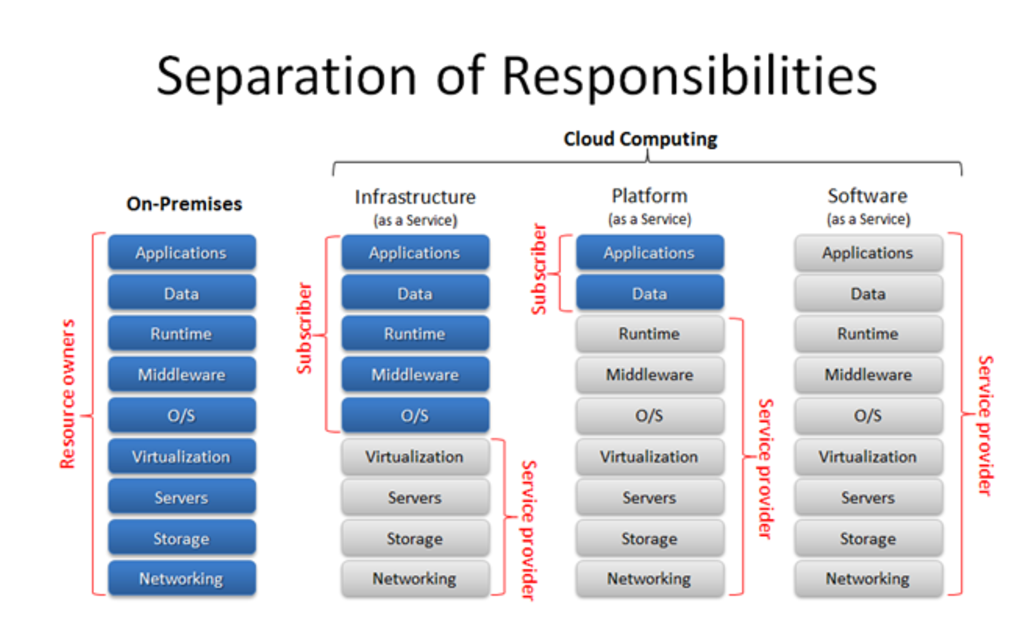
\includegraphics{graphics/service_models.eps}
	\caption{Service models\cite{trustedcloudcomputing}}
	\label{fig:cloud_stack}
\end{figure}

\todo{\url{https://blogs.technet.microsoft.com/yungchou/2010/11/15/cloud-computing-primer-for-it-pros/}}


Furthermore, the following subset of service models can be derived from the Everything as a Service (XaaS) aspect:

\subsubsection{Data Storage as a Service (DaaS)}
DaaS can be seen as enhancement of IaaS. The main idea behind this model is to provide storage solutions to users. Often supported services are databases (RDBMS or other types) and file storage.
		
Example: Amazon Simple Storage Service (S3)\cite{issues}.

\subsubsection{Human as a Service (HuaaS)}
Services, that rely on information generated by a crowd of people. Human intelligence is used to fulfill tasks that are provided as a service to the users. Persons in the crowd use their tools, skills or knowledge to solve a task or a small subset of a task. The cloud systems aggregates the single results and provide as a service to the users.
	
Example: Amazon Mechanical Turk\cite{huaas}.

\subsubsection{Other models}
Since there is no strict separation between the stated service models, there exist various combination and modifications of them. The following listing shows some additional classification \cite{cloud_characteristics}.
\begin{itemize}
	\item Database-as-a-Service
	\item Security-as-a-Service
	\item Communication-as-a-Service
	\item Management/Governance-as-a-Service
	\item Integration-as-a-Service
	\item Testing-as-a-Service
	\item Business Process-as-a-Service
\end{itemize}

\section{Internet of Things}

When looking at the past, a clear separation of digital and physical industries can be observerd. Since 1990, the Internet gave new opportunities to non-digital industries by creating new business models. Around 2005, the term ``Web 2.0'' came up as a summarization for Social Media, Open Source, Crowdsourcing, etc, allowing users to contribute to content in the Internet. With ``Web 3.0'' (around 2015), the concept of the ``Internet of Things (IoT)'' was introduced with new business models like ``Digitally Charged Products'' or ``Sensor as a Service'' \cite{iotfleisch}.

The Internet of Things introduces hybrid solutions that merge physical objects and digital services, with the vision to connect every object and location to the Internet. To fullfill this task, objects are equipped with computational intelligence (computers) that can be access over the Internet (or other objects) to read and write information from and to a physical object. The object itself is called a ``Thing'', hence the Name ``Internet of Things'' and is now a composition of both the physical and digital world \cite{iotfleisch}.

By adding computational intelligence to a physical object, the value of the ``Thing'' is increased in many ways. From an academic view, the value creation can be seen as five layers called the ``Value-creation Layers'' and will be explained in the next section \cite{iotfleisch}.

\url{https://www.alexandria.unisg.ch/236057/1/2090_EN_Bosch%20Lab%20White%20Paper%20GM%20im%20IOT%201_2.pdf}
\subsection{Value-creation Layers}

Figure \ref{fig:value_creation_layers} shows the five layers of value-creation within the Internet of Things. To get a better understanding of what the five layers are responsible for, a smart lightbulb is used as an example.

\begin{figure}[h]
	\centering
		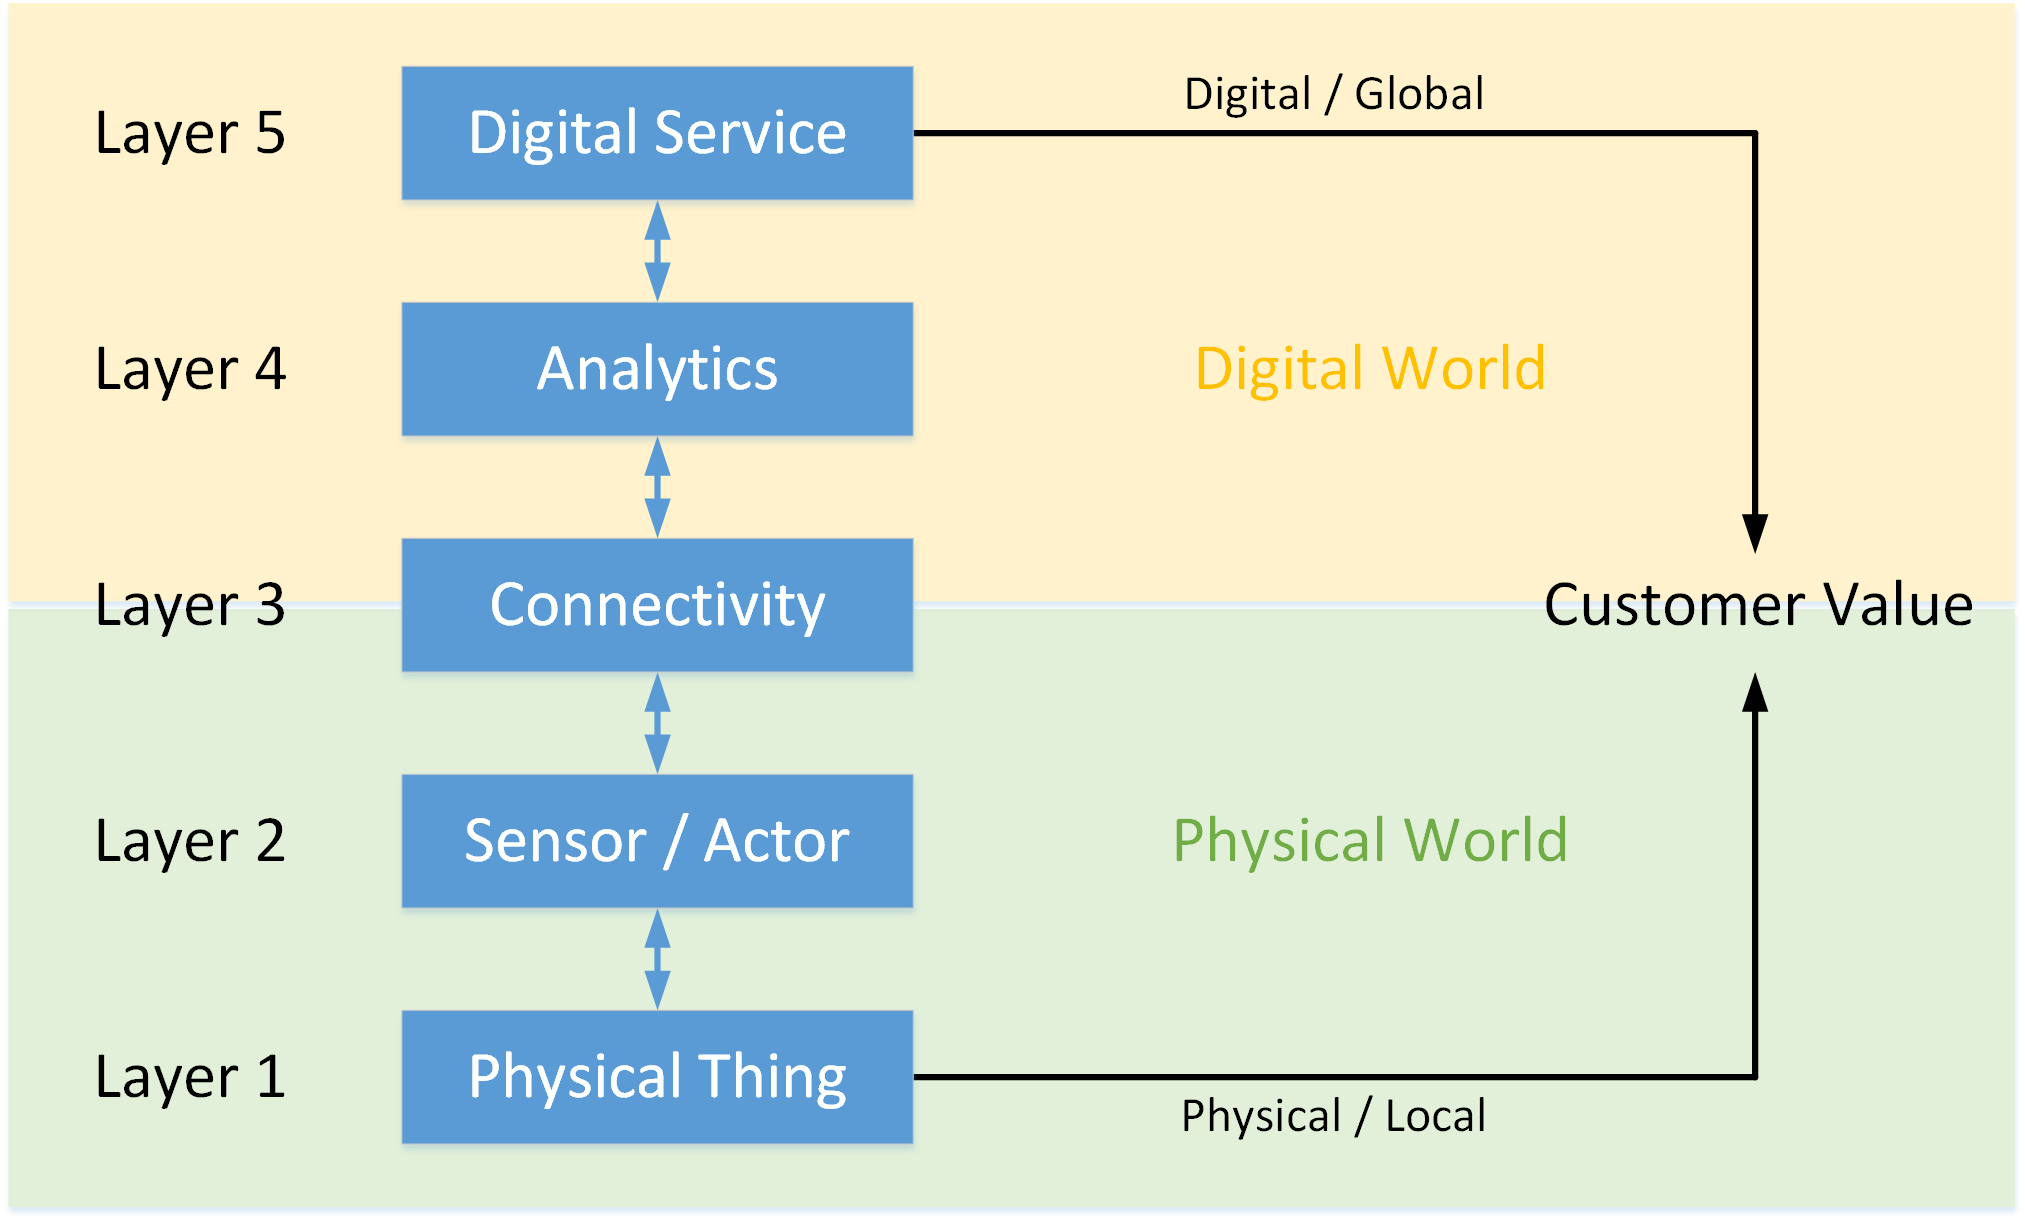
\includegraphics[scale=0.5]{graphics/iot_layers.eps}
	\caption{Value-creation Layers\cite{iotfleisch}}
	\label{fig:value_creation_layers}
\end{figure}

\subsubsection{Layer 1: Physical thing}
This layers describes the physical thing, e.g. a lightbulb. A thing is always bound to a location and has a direct benefit for the user (e.g. serving light). Since the location is fixed, it can only act in an immediate environment.

\subsubsection{Layer 2: Sensor/Actuator}
Layer 2 adds sensor and actuator elements to the thing. By adding a minicomputer to the physical object, the sensors can measure data and the actuators can deliver local services. In the proposed example, the sensor could measure the presense of a person and then switch of the lightbulb.

\subsubsection{Layer 3: Connectivity}
This layer connects the physical thing and the sensors/actuators to the Internet. Within this layer the device gets accessible via the Internet by, for example, a radio module that is connected to the local wireless network. By using modern technologies, this step can be done at marginal costs.

\subsubsection{Layer 4: Analytics}
In this layer, the collected data from the sensors are collected and stored for further processing (e.g. plausibility checks or classification). Additional web services can be integrated to generate actions for the actuators or add additional information to the sensor data. Usually this is achieved by using a cloud system. In this layer and additional value is added to the ``stupid'' thing. In the example this layer could derive motion patterns from the lightbulb.

\subsubsection{Layer 5: Digital service}
This layer combines all the previous layers and offers a functionality as a digital service. As an example, the lightbulb could be exposed to users all over the world via a wegbsite or a mobile application. On this layers new digital business model patterns can be applied.

By applying the previous layers to a physical object, the value of the thing is more than the sum of its parts. Connectivity to the Internet nowadays can be made at small costs. One important thing is, that the layers are not independent of each other. The flow of information has to pass the five layers always in both directions in order to ensure the additional value of the product.

\subsection{Business model patterns}

\subsection{Comparision with 'Industrial Internet of Things'}

\subsection{Comparision with 'Industry 4.0'}

\subsection{Impact on the thesis}
\todo{better title}


\chapter{System Design}
\section{Requirements}

\section{System Overview}

\section{Hardware Architecture}

\section{Software Architecture}

\subsection{Synchronization}
Synchronizing a distributed measurement system is essential. Although an not synchronized system delivers correct data that holds true for the point of measure, synchronizing theses systems allow to extract further knowledge out of the captured data. In the use case, selected for this thesis, power quality monitoring provides good arguments for synchronization. If somewhere in the power network an error occurs, it could be possible that this error is propagated throughout the network. Since the electric network and the infrastructure around it consists of resistive, inductive and capacitive load, a cascading of a fault is possible. With an adequate synchronization, it is possible to track the error propagation with a distributed measurement systems.

The testing equipment used in the proposed scenario support three different synchronization mechanisms. The radio based DCF77 time signal, the satellite based GPS signal and the Ethernet based SNTP protocol. The following section explains these three mechanisms in detail and evaluates which type suits most for this use case.

For the sake of completeness, two further synchronization modes exist. Distributed clock over EtherCAT and Q.sync. The first mode is part of the EtherCAT protocol that is implemented in the used modules, the second mode is a proprietary bus that connects multiple controllers. Since the different power quality measurement systems are spread across a wider geographical area, this two modes can't be used.

\subsubsection{DCF77}
DCF77 is a radio based time distribution services. It uses a long wave radio transmitter with a carrier frequency of 77.5 kHz. Due to the fact that the transmitter is located in Germany, it covers a maximum range (by using the proper detector) of approximately 2400 km, which is in fact whole Europe. Since DCF77 is driven by atomic clocks, the received radio signal is less accurate than the them\cite{dcf77}. Every minute, the time information (and additional information like civil warnings\cite{dcf77_2} and weather data\cite{dcf77}) is transmitted amplitude modulated (AM) and phase modulated (PM) in Binary Coded Decimal (BCD). In the current message the information about the next second is transmitted, furthermore, the start of a minute can be detected. It is possible to detect leap seconds and the switch to daylight-saving time \cite{dcf77_2}. Considering accuracy of the DCF77, the decoding mechanism is crucial. For the use in watches only the amplitude modulated signal is decoded which results in accuracy of +5ms up to +150ms. By using better antennas, this values can be enhanced to +5ms up to +15ms. To gain more accuracy, the phase modulated signal has to be decoded as well. This method results in an exactness of $\pm$2ms\cite{dcf77_3}.

Since the signal of a DCF77 receiver cannot be connected directly to the measurement devices, the signal has to be converter inside the receiver to a suitable format. As an example of such a format, the ''IRIG B003'' standard is described in more details here. The Inter Range Instrumentation Group (IRIG) specifies various standards regarding transmitting time information over via a serial time code format. The name of the described standard refers to a format with 100 pulses per second (B), Pulse width code (0), no carrier (0) and Binary Coded Decimal - BCD, Straight Binary Second of Day - SBS (3). The date information is transmitted as a sequence of seconds, minutes, hours, days, years, control functions and time of day \cite{irig}. Regarding the used testing equipment, DCF77 receivers can provide the IRIG B003 signal either straight as Transistor-Transistor Logic (TTL) signal into the measurement device, or over the RS-485 bus.

\subsubsection{GPS}
The Navstar Global Positioning System (GPS) is a satellite based time distribution service. In normal operation mode, it consists of 24 geometrical space slots with at least one operational satellite in it. Each satellite sends it's time information, generated by an atomic clock, and it's position to the receiver stations down on earth with a frequency of 1.57542 GHz. To control and observer the status of the GPS, the Operational Control System (OCS) is used to communicate with the satellites via ground antennas. The OCS is responsible for various tasks including telemetry, monitoring of different parameters and uploading of navigation data. Considering accuracy, GPS offers two services. On the one hand, the Standard Positioning Service (SPS) that is available to the civil public with less accuracy and on the other hand, the Precise Positioning Service (PPS) available to the military of the USA and it allies with high accuracy.\cite{gps}. Due to this fact, the proposed system and the used testing equipment can only make use of the SPS.

% genauigkeit, receiver, augmentation system

After receiving the time information from one or more satellites, the data can be passed to the testing equipment. For this, the received information is transformed to the National Marine Electronics Association (NMEA) 0183 format. Since NMEA was designed as interconnection format of different devices used in the marine, the format consists of various sentences representing features of the connected devices. To use NMEA as protocol for transmitting time- and position data, the two sentences \$GPRMC (Recommended Minimum Navigation Information) and \$GPGGA (Global Positioning System Fix Data. Time, Position and fix related data for a GPS receiver) can be used. The data is transferred as ASCII text and can be decoded directly by knowing the format of the corresponding sentence. NMEA uses, like IRIG, a serial bus for communication\cite{nmea}.

Beside NMEA, some GPS receivers are also able to provide information via the previously described IRIG B003 format.

\subsubsection{SNTP}
The Simple Network Time Protocol (SNTP), as a subset of the Network Time Protocol (NTP), provides time information in a network to clients. If a client wants to synchronize it's internal clock with a clock placed in the network (SNTP server), it has to send a message to this server. In the response, three timestamps are transmitted. The client timestamp when the message was sent, server time when the message was sent and server time when the message was received. With the information in this message and the timestamp when this message was received by the client, the exact time can be applied to the client\cite{sntp}. To synchronize a client's clock, the offset and delay of the client relative to the server is computed. By the used algorithm (especially because of the 64 bit integer arithmetic) a client has to be at least 34 years in the past and at most 34 years in future in order to get synchronized by the SNTP server\cite{rfc5905}.

%genauigkeit

\subsubsection{Conclusion}
\todo{add some content here}

\section{Network Architecture}


\section{Security Aspects / Threat-Modeling}
\todo{check spelling}

\chapter{Simulation}
\section{Tools}

\section{Test Data}
For testing purposes a set of prerecorded power data provided by the UK Energy Research Centre Energy Data Centre (UKERC-EDC) is used\cite{ukerc}.
This test set contains various types of data including 16 kHz recorded voltage and current values for a house in the UK, which will be used in the proposed thesis.

In chapter \ref{electric_characteristics} the optimal sample rate for measuring power quality parameters was calculated to be 20 kHz. Although the test data set has a sample rate of only 16 kHz, it can be used for simulation purposes. The slower sample rates result in a loss of information in the upper harmonics which have no big impact on the simulation, especially on the amount of data that has to be transferred from the measurement devices to the cloud system.

The recorded data is provided as flac-files\footnote{Free Lossless Audio Codec\cite{flac}}. Each file contains one hour of recording in a compressed format. The following procedure describes how to decode the values such that they can be used in the simulation environment.

\begin{enumerate}
	\item Convert flac-file to wav-file with sox\cite{sox}: \\ \lstinline[language=bash,basicstyle=\ttfamily]{sox.exe data.flac -e signed-integer -b 32 data.wav}
	\item Decode wav-file according to its specification\cite{wav}:
	\begin{enumerate}
		\item Deocode file header
		\item Decode data section
	\end{enumerate}
\end{enumerate}

The wav-files holds the values for voltage and current as consecutive 32-Bit-Integer values. First value is voltage, second is current and so on. These values has to be multiplied with calibration factors (also provided in the data sets) to get the real values for voltage and current. After this transformation, the values can be used in the simulation. Figure \ref{fig:test_data} shows an excerpt of the data after the transformation.

\begin{figure}[h]
	\centering
		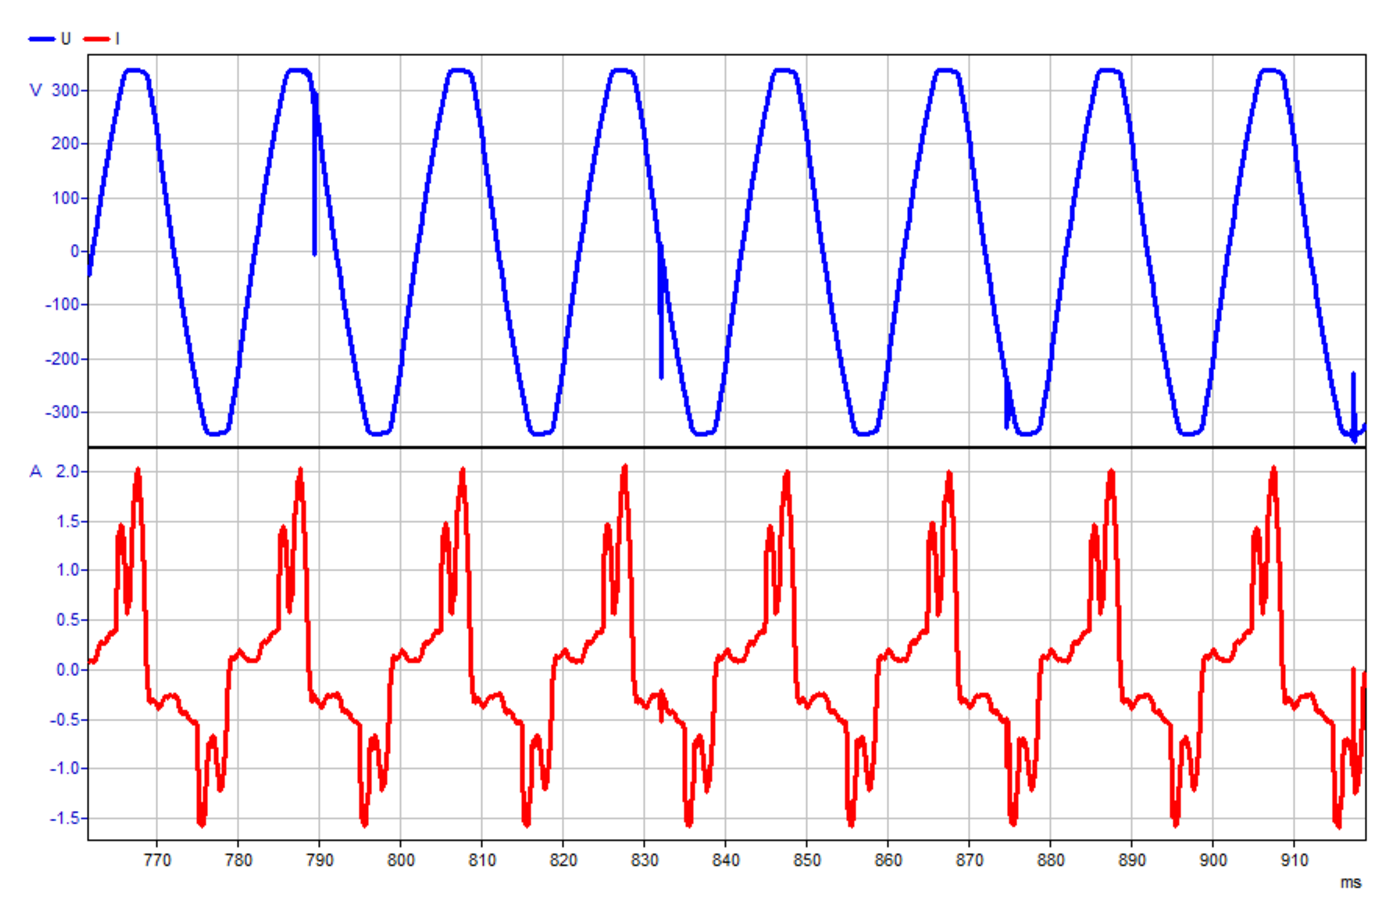
\includegraphics[scale=0.5]{graphics/testdata.eps}
	\caption{Test data}
	\label{fig:test_data}
\end{figure}

\section{Simulation Design}

Figure \ref{fig:simulation_design} shows the general simulation setup that is used to test the software components of the proposed system.

\begin{figure}[h]
	\centering
		\includegraphics[scale=0.7]{graphics/simulation_2.eps}
	\caption{Simulation design}
	\label{fig:simulation_design}
\end{figure}

Different parameters of the simulation can be changed, such that different environments can be simulated and evaluated against each other. The following enumeration describes the parameters that can be adapted as input data to the simulation:

\begin{itemize}
	\item Bandwidth of the Internet connection
		\begin{itemize}
			\item Wired connection: 100 MB/s, 50 MB/s, 20 MB/s, 10 MB/s
			\item WiFi connection: 
			\item Cellphone connection: LTE (), 4G (), 2G (), GPRS ()
		\end{itemize}
	\item Number of PQM meters
	\item Number of Webservices
	\item Transmitted data
		\begin{itemize}
			\item Raw data
			\item Preprocessed data
		\end{itemize}
  \item Storage
		\begin{itemize}
			\item File archive
			\item SQL database (MySQL)
			\item NoSQL database (CrateDB)
		\end{itemize}		
\end{itemize}

Modifications of the above mentioned parameters have an effect to the following parts:

\begin{itemize}
	\item Server side storage
	\item Network load, network costs
	\item Server side throughput
\end{itemize}

Table \ref{tab:SimulationResults} shows the expected results of the simulation:

\begin{table}[h]
\centering
\begin{tabular}{l|c|c|c|c}
\hline
\multicolumn{1}{l|}{\multirow{2}{*}{\textbf{Parameter}}} & \multicolumn{1}{c|}{\multirow{2}{*}{\textbf{Modification}}} & \multicolumn{3}{c}{\textbf{Impact}}                                                                                                  \\ \cline{3-5} 
\multicolumn{1}{c|}{} & \multicolumn{1}{c|}{}  & \multicolumn{1}{c|}{\textbf{Bandwidth}} & \multicolumn{1}{c|}{\textbf{Server storage}} & \multicolumn{1}{c}{\textbf{Throughput}} \\ \hline \hline
\multirow{2}{*}{\textbf{Bandwidth}} & \cellcolor{green} & \cellcolor{green} &\cellcolor{yellow}&\cellcolor{yellow}\\
\cline{2-5} 
                                                         & \cellcolor{red}                                                           & \cellcolor{red}                                       &\cellcolor{yellow}                                                &\cellcolor{yellow}                                      \\ \hline
\multirow{2}{*}{\textbf{Number of PQM meters}}           & \cellcolor{green}                                                           & \cellcolor{green}                                       & \cellcolor{green}                                                 & \cellcolor{red}                                       \\ \cline{2-5} 
                                                         & \cellcolor{red}                                                           & \cellcolor{red}                                       & \cellcolor{red}                                                 & \cellcolor{green}                                       \\ \hline
\multirow{2}{*}{\textbf{Number of web services}}          & \cellcolor{green}                                                           &\cellcolor{yellow}                                      &\cellcolor{yellow}                                                & \cellcolor{green}                                       \\ \cline{2-5} 
                                                         & \cellcolor{red}                                                           &\cellcolor{yellow}                                      &\cellcolor{yellow}                                                & \cellcolor{red}                                       \\ \hline
\multirow{2}{*}{\textbf{Transmitted Data}}               & \cellcolor{green}                                                           & \cellcolor{green}                                       & \cellcolor{green}                                                 & \cellcolor{red}                                       \\ \cline{2-5} 
                                                         & \cellcolor{red}                                                           & \cellcolor{red}                                       & \cellcolor{red}                                                 & \cellcolor{green}                                       \\ \hline
\multirow{3}{*}{\textbf{Server side storage}}            & File                                                        &\cellcolor{yellow}                                      & \cellcolor{purple}                                                 &\cellcolor{yellow}                                      \\ \cline{2-5} 
                                                         & SQL                                                         &\cellcolor{yellow}                                      & \cellcolor{purple}                                                 &\cellcolor{yellow}                                      \\ \cline{2-5} 
                                                         & NoSQL                                                       &\cellcolor{yellow}                                      & \cellcolor{purple}                                                 &\cellcolor{yellow}                                      \\ \hline
\end{tabular}
\caption{Simulation results}
\label{tab:SimulationResults}
\end{table}

\section{Evaluation}

\section{Impact on System Design}

\chapter{Implementation}
\input{chapters/impl}

\chapter{Evaluation}
\input{chapters/eval}



\backmatter

% Use an optional list of figures.
\listoffigures % Starred version, i.e., \listoffigures*, removes the toc entry.

% Use an optional list of tables.
\listoftables % Starred version, i.e., \listoftables*, removes the toc entry.

% Use an optional list of alogrithms.
\listofalgorithms
\addcontentsline{toc}{chapter}{List of Algorithms}

% Add an index.
\printindex

% Add a glossary.
\printglossaries

% Add a bibliography.
\bibliographystyle{unsrt}
\bibliography{intro}

\end{document}